\documentclass[a4paper,12pt]{article}

\usepackage[utf8x]{inputenc}
\usepackage[T2A]{fontenc}
\usepackage[english, russian]{babel}

% Опционно, требует  apt-get install scalable-cyrfonts.*
% и удаления одной строчки в cyrtimes.sty
% Сточку не удалять!
% \usepackage{cyrtimes}

% Картнки и tikz
\usepackage{graphicx}
\usepackage{tikz}
\usetikzlibrary{snakes,arrows,shapes}


% Некоторая русификация.
\usepackage{misccorr}
\usepackage{indentfirst}
\renewcommand{\labelitemi}{\normalfont\bfseries{--}}

% Увы, поля придётся уменьшить из-за листингов.
\topmargin -1cm
\oddsidemargin -0.5cm
\evensidemargin -0.5cm
\textwidth 17cm
\textheight 24cm

\sloppy

% Оглавление в PDF
\usepackage[
bookmarks=true,
colorlinks=true, linkcolor=black, anchorcolor=black, citecolor=black, menucolor=black,filecolor=black, urlcolor=black,
unicode=true
]{hyperref}

% Для исходного кода в тексте
\newcommand{\Code}[1]{\texttt{#1}}


\title{Отчёт по лабораторной работе \\ <<Динамическая IP-маршрутизация>>}
\author{Ермаков М.С. ИУ7-31М}

\begin{document}

\maketitle

\tableofcontents

\section{Настройка сети}

\subsection{Топология сети}

Топология сети и используемые IP-адреса показаны на рисунке~\ref{fig:network}.

\begin{figure}
\centering
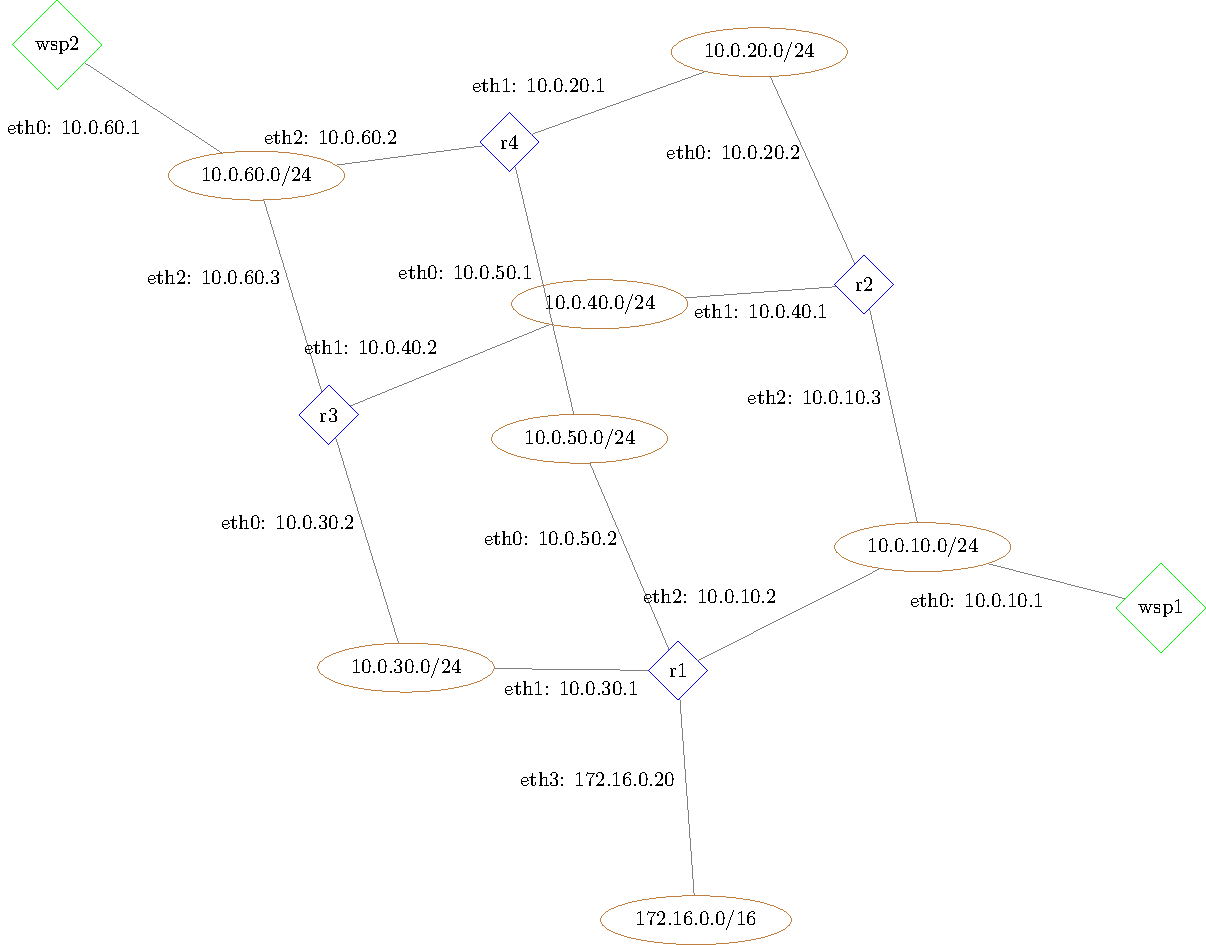
\includegraphics[width=0.8\textwidth]{includes/network_gv.pdf}
\caption{Топология сети}
\label{fig:network}
\end{figure}

Перечень узлов, на которых используется динамическая IP-маршрутизация:
r1, r2, r3, r4, wsp1, wsp2


\subsection{Назначение IP-адресов}

Ниже приведён файл сетевой настройки  маршрутизатора r1.

\begin{Verbatim}
    r1:~# cat /etc/network/interfaces 
    auto lo
    iface lo inet loopback
    
    auto eth0
    iface eth0 inet static
    address 10.0.50.2
    netmask 255.255.255.0
    
    auto eth1
    iface eth1 inet static
    address 10.0.30.1
    netmask 255.255.255.0
    
    auto eth2
    iface eth2 inet static
    address 10.0.10.2
    netmask 255.255.255.0
    
\end{Verbatim}

Ниже приведён файл сетевой настройки  маршрутизатора r2.

\begin{Verbatim}
    r2:~# cat /etc/network/interfaces 
    auto lo
    iface lo inet loopback
    
    auto eth0
    iface eth0 inet static
    address 10.0.20.2
    netmask 255.255.255.0
    
    auto eth1
    iface eth1 inet static
    address 10.0.40.1
    netmask 255.255.255.0
    
    auto eth2
    iface eth2 inet static
    address 10.0.10.3
    netmask 255.255.255.0    
\end{Verbatim}

Ниже приведён файл сетевой настройки  маршрутизатора r3.

\begin{Verbatim}
    r3:~# cat /etc/network/interfaces 
    auto lo
    iface lo inet loopback
    
    auto eth0
    iface eth0 inet static
    address 10.0.30.2
    netmask 255.255.255.0
    
    auto eth1
    iface eth1 inet static
    address 10.0.40.2
    netmask 255.255.255.0
    
    auto eth2
    iface eth2 inet static
    address 10.0.60.3
    netmask 255.255.255.0      
\end{Verbatim}

Ниже приведён файл сетевой настройки  маршрутизатора r4.

\begin{Verbatim}
    r4:~# cat /etc/network/interfaces 
    auto lo
    iface lo inet loopback
    
    auto eth0
    iface eth0 inet static
    address 10.0.50.1
    netmask 255.255.255.0
    
    auto eth1
    iface eth1 inet static
    address 10.0.20.1
    netmask 255.255.255.0
    
    auto eth2
    iface eth2 inet static
    address 10.0.60.2
    netmask 255.255.255.0         
\end{Verbatim}

Ниже приведён файл сетевой настройки рабочей станции wsp1.

\begin{Verbatim}
    wsp1:~# cat /etc/network/interfaces 
    auto lo
    iface lo inet loopback
    
    auto eth0
    iface eth0 inet static
    address 10.0.10.1
    netmask 255.255.255.0    
\end{Verbatim}

Ниже приведён файл сетевой настройки рабочей станции wsp2.

\begin{Verbatim}
    wsp2:~# cat /etc/network/interfaces 
    auto lo
    iface lo inet loopback
    
    auto eth0
    iface eth0 inet static
    address 10.0.60.1
    netmask 255.255.255.0    
\end{Verbatim}



\subsection{Настройка протокола RIP}

Ниже приведен файл \Code{/etc/quagga/ripd.conf} маршрутизатора r1.

\begin{Verbatim}
    r1:~# cat /etc/quagga/ripd.conf
    ! Этот настройки, касающиеся протокола RIP.
    router rip
    
    ! Раскомментируйте ниже все интерфейсы, подключённые
    ! к сетям с другими маршрутизаторами.
    network eth0
    network eth1
    network eth2
    ! network eth3
    
    ! Уменьшаем значения всех таймеров для ускорения опытов.
    ! Рассылка: 10 сек., устаревание: 60 cек., сборка мусора: 120 сек.
    timers basic 10 60 120
    
    ! Следующие две строчки заставляют маршрутизатор
    ! добавлять в сообщения протокола RIP все известные ему маршруты.
    redistribute kernel
    ! redistribute connected
    
    ! Это имя файла журнала службы RIP.
    ! Его содержимое можно изучить в случае неполадок
    log file /var/log/quagga/ripd.log
\end{Verbatim}

Ниже приведен файл \Code{/etc/quagga/ripd.conf} маршрутизатора r2.

\begin{Verbatim}
    r2:~# cat /etc/quagga/ripd.conf
    router rip
    
    network eth0
    network eth1
    network eth2
    
    timers basic 10 60 120

    redistribute kernel
    redistribute connected
    
    log file /var/log/quagga/ripd.log
    
\end{Verbatim}

Ниже приведен файл \Code{/etc/quagga/ripd.conf} маршрутизатора r3.

\begin{Verbatim}
    r3:~# cat /etc/quagga/ripd.conf
    router rip
    
    network eth0
    network eth1
    network eth2
    
    timers basic 10 60 120

    redistribute kernel
    redistribute connected
    
    log file /var/log/quagga/ripd.log
\end{Verbatim}

Ниже приведен файл \Code{/etc/quagga/ripd.conf} маршрутизатора r4.

\begin{Verbatim}
    r4:~# cat /etc/quagga/ripd.conf
    router rip
    
    network eth0
    network eth1
    network eth2
    
    timers basic 10 60 120

    redistribute kernel
    redistribute connected
    
    log file /var/log/quagga/ripd.log
\end{Verbatim}


Ниже приведен файл \Code{/etc/quagga/ripd.conf} рабочий станции, связанной с несколькими маршрутизаторами wsp1.

\begin{Verbatim}
    wsp1:~# cat /etc/quagga/ripd.conf
    router rip
    
    network eth0
    
    timers basic 10 60 120

    redistribute kernel
    redistribute connected
    
    log file /var/log/quagga/ripd.log
\end{Verbatim}

Ниже приведен файл \Code{/etc/quagga/ripd.conf} рабочий станции, связанной с несколькими маршрутизаторами wsp2.

\begin{Verbatim}
    wsp1:~# cat /etc/quagga/ripd.conf
    router rip
    
    network eth0
    
    timers basic 10 60 120

    redistribute kernel
    redistribute connected
    
    log file /var/log/quagga/ripd.log
\end{Verbatim}


\section{Проверка настройки протокола RIP}

Вывод \textbf{traceroute} от узла wsp1 до wsp2 при нормальной работе сети.

\begin{Verbatim}
    wsp1:~# traceroute -n 10.0.60.1
    traceroute to 10.0.60.1 (10.0.60.1), 64 hops max, 40 byte packets
     1  10.0.10.2  1 ms  0 ms  0 ms
     2  10.0.30.2  11 ms  1 ms  1 ms
     3  10.0.60.1  12 ms  1 ms  1 ms
\end{Verbatim}

Вывод \textbf{traceroute} от узла такого-то до внешнего IP.

\begin{Verbatim}
    r1:~# traceroute -n 194.190.254.106
    traceroute to 194.190.254.106 (194.190.254.106), 64 hops max, 40 byte packets
     1  172.16.0.1  0 ms  0 ms  0 ms
     2  192.168.0.1  3 ms  1 ms  1 ms
     3  192.168.1.254  2 ms  3 ms  2 ms
     4  100.103.0.1  6 ms  6 ms  6 ms
     5  212.188.1.6  7 ms  12 ms  12 ms
     6  212.188.1.5  6 ms (TOS=32!)  6 ms *
     7  * 195.34.53.206 [MPLS: Label 100219 Exp 1]  7 ms  8 ms
     8  212.188.28.102 [MPLS: Label 100221 Exp 1]  6 ms  6 ms  7 ms
     9  195.34.53.204  7 ms  6 ms  6 ms
    10  212.188.33.181  5 ms  6 ms  6 ms
    11  194.190.254.106  6 ms *  7 ms    
\end{Verbatim}

Вывод сообщения RIP, перехваченного на маршрутизаторе r3.

\begin{Verbatim}
r3:~# tcpdump -tvn -i eth0 -s 1518 udp
tcpdump: listening on eth0, link-type EN10MB (Ethernet), capture size 1518 bytes
IP (tos 0x0, ttl 1, id 0, offset 0, flags [DF], proto UDP (17), length 92) 10.0.30.2.520 > 224.0.0.9.520: 
	RIPv2, Response, length: 64, routes: 3
	  AFI: IPv4:       10.0.20.0/24, tag 0x0000, metric: 2, next-hop: self
	  AFI: IPv4:       10.0.40.0/24, tag 0x0000, metric: 1, next-hop: self
	  AFI: IPv4:       10.0.60.0/24, tag 0x0000, metric: 1, next-hop: self
IP (tos 0x0, ttl 1, id 0, offset 0, flags [DF], proto UDP (17), length 112) 10.0.30.1.520 > 224.0.0.9.520: 
	RIPv2, Response, length: 84, routes: 4
	  AFI: IPv4:         0.0.0.0/0 , tag 0x0000, metric: 1, next-hop: self
	  AFI: IPv4:       10.0.10.0/24, tag 0x0000, metric: 1, next-hop: self
	  AFI: IPv4:       10.0.20.0/24, tag 0x0000, metric: 2, next-hop: self
	  AFI: IPv4:       10.0.50.0/24, tag 0x0000, metric: 1, next-hop: self
\end{Verbatim}

Вывод таблицы RIP.

\begin{Verbatim}
r3# show ip rip
Codes: R - RIP, C - connected, S - Static, O - OSPF, B - BGP
Sub-codes:
      (n) - normal, (s) - static, (d) - default, (r) - redistribute,
      (i) - interface

     Network            Next Hop         Metric From            Tag Time
R(n) 0.0.0.0/0          10.0.30.1             2 10.0.30.1         0 00:51
R(n) 10.0.10.0/24       10.0.30.1             2 10.0.30.1         0 00:51
R(n) 10.0.20.0/24       10.0.40.1             2 10.0.40.1         0 00:58
C(i) 10.0.30.0/24       0.0.0.0               1 self              0
C(i) 10.0.40.0/24       0.0.0.0               1 self              0
R(n) 10.0.50.0/24       10.0.30.1             2 10.0.30.1         0 00:51
C(i) 10.0.60.0/24       0.0.0.0               1 self              0
\end{Verbatim}

Вывод таблицы маршрутизации.

\begin{Verbatim}
r3:~# ip r
10.0.20.0/24 via 10.0.40.1 dev eth1  proto zebra  metric 2 
10.0.50.0/24 via 10.0.30.1 dev eth0  proto zebra  metric 2 
10.0.60.0/24 dev eth2  proto kernel  scope link  src 10.0.60.3 
10.0.30.0/24 dev eth0  proto kernel  scope link  src 10.0.30.2 
10.0.40.0/24 dev eth1  proto kernel  scope link  src 10.0.40.2 
10.0.10.0/24 via 10.0.30.1 dev eth0  proto zebra  metric 2 
default via 10.0.30.1 dev eth0  proto zebra  metric 2 
\end{Verbatim}

\section{Расщепленный горизонт и испорченные обратные обновления}

Поместить сюда вывод сообщения одного и того же маршрутизатор с включенным расщ. горизонтом, с включенными испорченными обновлениями, с отключённым расщ. гор.

Объяснить разницу.

Вернуть настройки в исходное состояние (включенный без испорченных).

Перехват сообщений RIP с включенным расщипленным горизонтом.

\begin{Verbatim}
r3:~# tcpdump -tvn -i eth0 -s 1518 udp
tcpdump: listening on eth0, link-type EN10MB (Ethernet), capture size 1518 bytes
IP (tos 0x0, ttl 1, id 0, offset 0, flags [DF], proto UDP (17), length 92) 10.0.30.2.520 > 224.0.0.9.520: 
	RIPv2, Response, length: 64, routes: 3
	  AFI: IPv4:       10.0.20.0/24, tag 0x0000, metric: 2, next-hop: self
	  AFI: IPv4:       10.0.40.0/24, tag 0x0000, metric: 1, next-hop: self
	  AFI: IPv4:       10.0.60.0/24, tag 0x0000, metric: 1, next-hop: self
IP (tos 0x0, ttl 1, id 0, offset 0, flags [DF], proto UDP (17), length 112) 10.0.30.1.520 > 224.0.0.9.520: 
	RIPv2, Response, length: 84, routes: 4
	  AFI: IPv4:         0.0.0.0/0 , tag 0x0000, metric: 1, next-hop: self
	  AFI: IPv4:       10.0.10.0/24, tag 0x0000, metric: 1, next-hop: self
	  AFI: IPv4:       10.0.20.0/24, tag 0x0000, metric: 2, next-hop: self
	  AFI: IPv4:       10.0.50.0/24, tag 0x0000, metric: 1, next-hop: self
\end{Verbatim}

Перехват сообщений RIP с включенным испорченным обновлением

\begin{Verbatim}
r3:~# tcpdump -tvn -i eth0 -s 1518 udp
tcpdump: listening on eth0, link-type EN10MB (Ethernet), capture size 1518 bytes
IP (tos 0x0, ttl 1, id 0, offset 0, flags [DF], proto UDP (17), length 112) 10.0.30.1.520 > 224.0.0.9.520: 
	RIPv2, Response, length: 84, routes: 4
	  AFI: IPv4:         0.0.0.0/0 , tag 0x0000, metric: 1, next-hop: self
	  AFI: IPv4:       10.0.10.0/24, tag 0x0000, metric: 1, next-hop: self
	  AFI: IPv4:       10.0.20.0/24, tag 0x0000, metric: 2, next-hop: self
	  AFI: IPv4:       10.0.50.0/24, tag 0x0000, metric: 1, next-hop: self
IP (tos 0x0, ttl 1, id 0, offset 0, flags [DF], proto UDP (17), length 172) 10.0.30.2.520 > 224.0.0.9.520: 
	RIPv2, Response, length: 144, routes: 7
	  AFI: IPv4:         0.0.0.0/0 , tag 0x0000, metric: 16, next-hop: 10.0.30.1
	  AFI: IPv4:       10.0.10.0/24, tag 0x0000, metric: 16, next-hop: 10.0.30.1
	  AFI: IPv4:       10.0.20.0/24, tag 0x0000, metric: 2, next-hop: self
	  AFI: IPv4:       10.0.30.0/24, tag 0x0000, metric: 16, next-hop: self
	  AFI: IPv4:       10.0.40.0/24, tag 0x0000, metric: 1, next-hop: self
	  AFI: IPv4:       10.0.50.0/24, tag 0x0000, metric: 16, next-hop: 10.0.30.1
	  AFI: IPv4:       10.0.60.0/24, tag 0x0000, metric: 1, next-hop: self
\end{Verbatim}

Перехват сообщений с отключенным расщипленным горизонтом

\begin{Verbatim}
r3:~# tcpdump -tvn -i eth0 -s 1518 udp
tcpdump: listening on eth0, link-type EN10MB (Ethernet), capture size 1518 bytes
IP (tos 0x0, ttl 1, id 0, offset 0, flags [DF], proto UDP (17), length 112) 10.0.30.1.520 > 224.0.0.9.520: 
	RIPv2, Response, length: 84, routes: 4
	  AFI: IPv4:         0.0.0.0/0 , tag 0x0000, metric: 1, next-hop: self
	  AFI: IPv4:       10.0.10.0/24, tag 0x0000, metric: 1, next-hop: self
	  AFI: IPv4:       10.0.20.0/24, tag 0x0000, metric: 2, next-hop: self
	  AFI: IPv4:       10.0.50.0/24, tag 0x0000, metric: 1, next-hop: self
IP (tos 0x0, ttl 1, id 0, offset 0, flags [DF], proto UDP (17), length 172) 10.0.30.2.520 > 224.0.0.9.520: 
	RIPv2, Response, length: 144, routes: 7
	  AFI: IPv4:         0.0.0.0/0 , tag 0x0000, metric: 2, next-hop: 10.0.30.1
	  AFI: IPv4:       10.0.10.0/24, tag 0x0000, metric: 2, next-hop: 10.0.30.1
	  AFI: IPv4:       10.0.20.0/24, tag 0x0000, metric: 2, next-hop: self
	  AFI: IPv4:       10.0.30.0/24, tag 0x0000, metric: 1, next-hop: self
	  AFI: IPv4:       10.0.40.0/24, tag 0x0000, metric: 1, next-hop: self
	  AFI: IPv4:       10.0.50.0/24, tag 0x0000, metric: 2, next-hop: 10.0.30.1
	  AFI: IPv4:       10.0.60.0/24, tag 0x0000, metric: 1, next-hop: self
\end{Verbatim}

\section{Имитация устранимой поломки в сети}



Отлючили маршрутизатор r2

Вывод таблицы RIP непосредственно перед истечением таймера устаревания на маршрутизаторе r3.
До отключение маршрутизатора r2 маршрут к сети 10.0.20.0 на машине r3 проходил через  10.0.40.1

\begin{Verbatim}
r3# show ip rip
Codes: R - RIP, C - connected, S - Static, O - OSPF, B - BGP
Sub-codes:
      (n) - normal, (s) - static, (d) - default, (r) - redistribute,
      (i) - interface

     Network            Next Hop         Metric From            Tag Time
R(n) 10.0.10.0/24       10.0.30.1             2 10.0.30.1         0 00:58
R(n) 10.0.20.0/24       10.0.40.1             2 10.0.40.1         0 00:42
C(i) 10.0.30.0/24       0.0.0.0               1 self              0
C(i) 10.0.40.0/24       0.0.0.0               1 self              0
R(n) 10.0.50.0/24       10.0.30.1             2 10.0.30.1         0 00:58
C(i) 10.0.60.0/24       0.0.0.0               1 self              0

\end{Verbatim}

После истекания таймера устаревания новый путь до сети 10.0.20.0 проходит через 10.0.60.2

Перестроенная таблица на этом же маршрутизаторе

\begin{Verbatim}
r3# show ip rip
Codes: R - RIP, C - connected, S - Static, O - OSPF, B - BGP
Sub-codes:
      (n) - normal, (s) - static, (d) - default, (r) - redistribute,
      (i) - interface

     Network            Next Hop         Metric From            Tag Time
R(n) 10.0.10.0/24       10.0.30.1             2 10.0.30.1         0 00:53
R(n) 10.0.20.0/24       10.0.60.2             2 10.0.60.2         0 00:59
C(i) 10.0.30.0/24       0.0.0.0               1 self              0
C(i) 10.0.40.0/24       0.0.0.0               1 self              0
R(n) 10.0.50.0/24       10.0.30.1             2 10.0.30.1         0 00:53
C(i) 10.0.60.0/24       0.0.0.0               1 self              0
\end{Verbatim}


Вывод \textbf{traceroute} от узла wsp1 до wsp2 после того, как служба RIP перестроила таблицы маршрутизации.

\begin{Verbatim}
wsp1:~# traceroute -n 10.0.60.1
traceroute to 10.0.60.1 (10.0.60.1), 64 hops max, 40 byte packets
 1  10.0.10.2  1 ms  0 ms  0 ms
 2  10.0.50.1  4 ms  0 ms  0 ms
 3  10.0.60.1  18 ms  2 ms  2 ms
\end{Verbatim}

\section{Имитация неустранимой поломки в сети}

Выключили маршрутизатор r4, тем самым отрезали путь от r3 до сети 10.0.20.0

Далее поместить таблицы протокола RIP, где видна 16-ая метрика, и сообщения протокола RIP с 16-ой метрикой.

Путь до сети 10.0.20.0 через 10.0.60.2 теперь стал иметь метрику равную 16 (бесконечность)

Таблица RIP

\begin{Verbatim}
r3# show ip rip
Codes: R - RIP, C - connected, S - Static, O - OSPF, B - BGP
Sub-codes:
      (n) - normal, (s) - static, (d) - default, (r) - redistribute,
      (i) - interface

     Network            Next Hop         Metric From            Tag Time
R(n) 10.0.10.0/24       10.0.30.1             2 10.0.30.1         0 00:51
R(n) 10.0.20.0/24       10.0.60.2            16 10.0.60.2         0 01:47
C(i) 10.0.30.0/24       0.0.0.0               1 self              0
C(i) 10.0.40.0/24       0.0.0.0               1 self              0
R(n) 10.0.50.0/24       10.0.30.1             2 10.0.30.1         0 00:51
C(i) 10.0.60.0/24       0.0.0.0               1 self              0
\end{Verbatim}

tcpdump на машине r3

\begin{Verbatim}
r3:~# tcpdump -tvn -i eth0 -s 1518 udp
tcpdump: listening on eth0, link-type EN10MB (Ethernet), capture size 1518 bytes
IP (tos 0x0, ttl 1, id 0, offset 0, flags [DF], proto UDP (17), length 92) 10.0.30.2.520 > 224.0.0.9.520: 
	RIPv2, Response, length: 64, routes: 3
	  AFI: IPv4:       10.0.20.0/24, tag 0x0000, metric: 16, next-hop: self
	  AFI: IPv4:       10.0.40.0/24, tag 0x0000, metric: 1, next-hop: self
	  AFI: IPv4:       10.0.60.0/24, tag 0x0000, metric: 1, next-hop: self
IP (tos 0x0, ttl 1, id 0, offset 0, flags [DF], proto UDP (17), length 92) 10.0.30.1.520 > 224.0.0.9.520: 
	RIPv2, Response, length: 64, routes: 3
	  AFI: IPv4:       10.0.10.0/24, tag 0x0000, metric: 1, next-hop: self
	  AFI: IPv4:       10.0.20.0/24, tag 0x0000, metric: 16, next-hop: self
	  AFI: IPv4:       10.0.50.0/24, tag 0x0000, metric: 1, next-hop: self
\end{Verbatim}

\end{document}

